\documentclass[a4paper]{article}

\usepackage[english]{babel}
\usepackage[utf8]{inputenc}
\usepackage[hidelinks]{hyperref}

\usepackage{graphicx}
\graphicspath{ {images/} }

\usepackage{floatrow}
\thisfloatsetup{
  capposition=beside,
  capbesideposition={bottom,right},
  capbesidewidth=.3\textwidth,
  justification=raggedright
}

\usepackage{setspace}
\usepackage{pdfpages}
\usepackage{xspace} %Removes space after commands
\usepackage{fancyhdr}
\usepackage{lastpage}
\usepackage{verbatim}
\usepackage{url}

%%% BibTeX %%%
\usepackage{cite}
% JS function to get BibTeX entry from WebAssembly website
\begin{comment}
function BibTeX() {
	let subject = document.title.replace(/ - WebAssembly/, '').replace(' ', '-').toLowerCase();
    return `@misc{website:wasm-${subject}
	author = "The WebAssembly working group",
	title = {{${document.title}}},
	url = "${document.URL}",
	note = {Online; accessed 3 May 2017},
}`;
}
\end{comment}

% source: https://tex.stackexchange.com/a/35044
\makeatletter
\newcommand\footnoteref[1]{\protected@xdef\@thefnmark{\ref{#1}}\@footnotemark}
\makeatother

% Code highlighting
\usepackage{minted}
% Highlight theme
\usemintedstyle{trac}

\pagestyle{fancy}
\fancyhf{}

\lfoot{Page \thepage \hspace{1pt} of \pageref{LastPage}}

\usepackage[margin=0.8in]{geometry}

\title{Bachelor Project Report: Compiling MicroC to WebAssembly}

\begin{document}
%\pagenumbering{gobble} %Remove page numbers
\begin{titlepage}
	\centering
	{\scshape\LARGE IT University of Copenhagen \par}
	\vspace{1cm}
	{\scshape\Large Bachelor Project Report\par}
	\vspace{1.5cm}
	{\huge\bfseries Compiling MicroC to WebAssembly \par}
	\vspace{2cm}
	{
\includegraphics{WebAssemblyLogo} \par}
	\vspace{2cm}
	{\Large\itshape Andreas Bjørn Hassing Nielsen\par}
	abhn@itu.dk\\
	\vspace{2cm}
	{\Large Abstract\par}
	%TODO: Write an awesome abstract.
	{\bfseries This is where the abstract will go.}
	\vfill
% Bottom of the page
	{\large \today\par}
\end{titlepage}

\newpage

\tableofcontents
\newpage


\section{Introduction}
The purpose of this project is to build a compiler, also called a translator, from MicroC to WebAssembly, using FsLexYacc\footnote{\label{footnote:fslexyacc-url}http://fsprojects.github.io/FsLexYacc/} and F\#\footnote{http://fsharp.org/}. The learning goals are to develop an understanding of WebAssembly and improve my knowledge of compiler design.

MicroC is a C-like language described by Peter Sestoft in the book Programming Language Concepts~\cite{PLC}. The original lexer and parser code can be found at his website\footnote{http://www.itu.dk/people/sestoft/plc/}.

\section{Problem Definition}
WebAssembly (WASM) is a new up-and-coming binary code format for the user-facing web, designed to work alongside JavaScript as a more portable, size- and load-time-efficient, ahead-of-time-compiled alternative. 

The binary WASM format is not bound to be emitted by JavaScript (asm.js) only, potentially bringing your favourite language to the browser front-end. If a language can compile to a intermediate representation supported by WASM (LLVM IR, for instance), it can be compiled to the binary WASM format. 

The purpose of this project is to shed some light on the unfinished WebAssembly specification. To assist in meeting this goal, a compiler will be designed, that compiles from a simple programming language, MicroC, to a WASM format that can be run in a WASM-enabled browser today (currently requiring Firefox Nightly or Chrome Canary with WASM flags set to enabled\footnote{At the time of writing (May, 2017), setting flags or using a nightly browser version is no longer required. Major browsers now support WASM out of the box: https://lists.w3.org/Archives/Public/public-webassembly/2017Feb/0002.html}).

\subsection{Method}
What follows is the planned activities and sources of information.
\begin{itemize}
	\item Translation of MicroC to the binary WebAssembly format, using FsLexYacc\footnoteref{footnote:fslexyacc-url}, as used in the Programs as Data course (fall 2016).
	\item Course books from Programs as Data (fall 2016) will be used as knowledge base for MicroC to WebAssembly translation:
		\begin{itemize}
			\item Peter Sestoft: Programming Language Concepts. Springer 2012.
			\item Torben Mogensen: Basics of Compiler Design. DIKU 2010. Chapters 2 and 3.
		\end{itemize}
	\item Knowledge of WebAssembly will be gained through the official website (http://webassembly.org/) and links branching out from it.
	\item Creation of prototype: web interface that lets users type MicroC in a window, and see it generate WebAssembly in some human-readable format, either s-expression or linear bytecode. The prototype will also give users the ability to run their code as WebAssembly, given that the browser in use supports it.
	\item Reflection over, either the security behind WebAssembly or the portability of it between browsers and platforms.
\end{itemize}

\noindent If time allows:
\begin{itemize}
	\item Extensions to the MicroC language will be implemented.
	\item Simple optimizations to the generated WebAssembly code.
\end{itemize}
\pagebreak

\section{Problem Analysis}
In this section, the problem will be dissected and analysed. The definition of a compiler is defined and the WebAssembly specification and binary encoding is scrutinised.

\subsection{Compilers in General}
Before the compiler design is even considered, an important, and perhaps trivial, question must be asked and answered: "What is a compiler?".

According to the definition laid out by Mogensen~\cite{BCD}, a compiler is a program that takes the source code of another program as input, usually some higher-level language such as C\#, and compiles it to a lower-level representation, Common Intermediate Language code - in the case of C\#, or binary machine code instructions - in the case of C. There are more low-level representations out in the wild, but these two will be the ones referenced in this report.

Many programs are written in higher-level languages that run within an assisting runtime environment and compiles to a variant of bytecode, with an instruction set specified in the virtual machine of the runtime. When the runtime is started and the program bytecode is passed to it, it performs a just-in-time (JIT) compilation to native machine code using the instruction set of the machine's processor. The .NET CLR and Java's JRE are two such runtimes that both support several higher-level languages, such as C\#, F\#, Java and Scala. Runtime environments often come equipped with integrated memory management in the form of a garbage collector.

Programs written in comparatively lower-level languages, such as C and C++, are usually compiled ahead-of-time (AOT) to native machine code using the instruction set of the compiling machine. One can often configure the compiler to target other operating systems and processor architectures than that of the compiling system. In these lower-level languages, the programmer is often challenged with manually managing dynamic memory.

Note, that nothing stops us from implementing a runtime environment that supports a high-level language, such as C, which can then run code written in that language as a JIT compiled application. The task may be non-trivial.

Then, there is JavaScript, a loosely typed language that runs in browsers. JavaScript is compiled by a JIT compiler at runtime\footnote{This is not always true. Ignition, a newly developed interpreter for V8 (Chrome's JavaScript engine), is used alone or along with JIT compilation, especially on devices where a lower- memory footprint, or battery usage is beneficial (Smartphones, for instance)~\cite{video:thompson-js-perf-v8-and-wasm}.}, which takes the code, turns it into abstract syntax and then to machine code~\cite[p.~13]{slides:lund-v8}. During the execution of a JavaScript program, the JIT compiler will attempt to optimise the generated machine code by making probabilistic assumptions about program behaviour. These assumptions can eventually fail, thus forcing the JIT to throw away optimisations based on falsified claims - this is a cause of non-deterministic execution speed of JavaScript programs. The JIT's that are found in modern browsers make a lot of intelligent optimisations on what is generally referred to as \texttt{warm} and \texttt{hot} code paths\footnote{Warm and hot code, is code segments that are executed regularly, and often, respectively.}, thereby greatly increasing performance without sacrificing excessive resources. When a JIT compiler is run on a system with multiple processor cores, it can run in parallel, thereby generating optimisations without blocking the main thread of the program.

\subsubsection{Benefits of AOT Compilation}
\textbf{Static Type Checking} When a statically typed language is compiled ahead-of-time, the compiler can complain to the developer before the program hits runtime. For instance, if the developer attempts to assign a char value to a variable that is declared to contain an integer, the compilation will fail. This is useful for producing correct code. JavaScript is a loosely typed language, meaning that type checking happens late, and errors that didn't show during development, can show up in the users browser.\\

\noindent \textbf{Optimisations} While optimisations can be made by both an AOT and JIT compiler, an AOT has all the time a developer has to spare, to optimise. A JIT will need to weigh the potential gain of an optimisation against slowing down the program during the consideration process. This makes an AOT compiler preferred for live- and runtime critical systems.

%TODO: add more to AOT benefits?
%TODO: add JIT benefits?

\subsection{WebAssembly}

\subsection{History}
There was only 1 language that could run natively in all browsers less than a year ago: JavaScript. The web is built around it, and the language has flourished and expanded beyond the land of browsers, in the form of execution environments such as Node.js\footnote{https://nodejs.org/} and native application frameworks such as React Native\footnote{https://facebook.github.io/react-native/} and Electron\footnote{https://electron.atom.io/}.

JavaScript is a loosely typed language, meaning that types are checked at runtime, such that . This fact takes away some performance as the program runs. This happens because, the JIT compiler that backs JavaScript in browsers will attempt to derive what types variables and functions have in the running program, in order to make some type-check reducing optimisations, but may end up being wrong and discarding them again~\cite{video:thompson-js-perf-v8-and-wasm}.

\section{User Guide and Examples}

\section{Technical Description}

\section{Testing and Validation}

\section{Peripheral Programs and Tooling}
This section describes the use of peripheral programs and tooling that assist in, compiling the compiler, or exposing the generated code from compiled MicroC programs.



\section{Future Extensions}

\subsection{Compiler Optimisations}
Humans (should) write readable and maintainable code. A computer only cares about operations, and each operation costs some $x$ energy and time. The compiler can perform optimisations to reduce the amount of operations a program needs for some logic to be completed, this machine code reduction positively influences the compiled program, by reducing the energy consumed by a processor running it, and increasing the performance.

\textbf{Peephole optimisation} is a simple technique that consumes few resources and little time. The cause of this is that peephole optimisations only require knowledge of a few close operations in order to apply reductions.

\begin{figure}[H]
	\floatbox{figure}[\FBwidth]{\caption{A simple function \texttt{optEx} multiplies the input argument with $0$ a few times and then returns the result of an addition. To the right of the function are the compiled and optimised versions of the code in WebAssembly stack machine code.}}
	{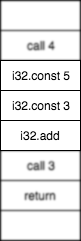
\includegraphics[width=0.1\textwidth]{PeepholeOptimisationIllustration}}
	\centering
\end{figure}

In a forward compiler, optimising with peephole style optimisations can be added as a pass in the backend compiler, such that when the instruction code is generated, the compiler will run through it again, this time attempting to apply optimisations which attempts to reduce and remove code. For instance, if a function in a program adds two constants together and returns the result, an optimising compiler will reduce the expression to the result of the addition operation, and simply return that: \mintinline{c}{return 7+14; => return 21;}. The logic has not been tampered with, but the function is now an operation cheaper. A more elaborate example can be found below.

\begin{figure}[H]
	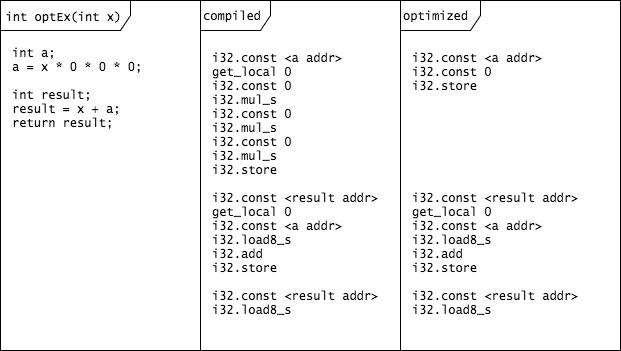
\includegraphics[width=0.75\textwidth]{PeepholeOptimisation}
	\centering
	\caption{A simple function \texttt{optEx} multiplies the input argument with $0$ a few times and then returns the result of an addition. To the right of the function are the compiled and optimised versions of the code in WebAssembly stack machine code.}
\label{fig:peephole-optimisation}
\end{figure}
As can be seen in figure~\ref{fig:peephole-optimisation}, only the multiplication expressions are simplified. While peephole optimising, the compiler will not know if it can discard \texttt{a} entirely, as it could be referenced later, and the compiler does not know the value of \texttt{x}, nor what \texttt{a} contains anymore (we can see that it is equal to $0$, but our brains collect a lot of state regarding the program at hand, which allows us to deduce this), therefore, nothing can be optimised at the end of the function. Running a more complex and stateful optimisation technique could detect more redundant code, but such an optimisation is more resource- and time consuming.

Peephole optimisations fall short when more elaborate optimisations are needed. For instance, if you have many small functions you may want to inline them where used. If we reuse the example from above, with the add function, simply adding the result to the stack rather than calling the function each place is fewer operations, thus inlining would yield a benefit. During peephole optimisation, you won't have information regarding the environment, thus you won’t know what the function that is being called will do, and will not know if inlining is legal.

\section{Conclusion}

\section{References}
\begingroup
\renewcommand{\section}[2]{}%
\bibliographystyle{plain}
\bibliography{Bibliography}{}
\endgroup

\section{Appendix}

\end{document}
